\section{Problem 3}

\subsection{Question}
\vspace*{10pt}
Estimate the age of each of the 1000 URIs using the \enquote{Carbon Date} tool:\\
\\
http://ws-dl.blogspot.com/2014/11/2014-11-14-carbon-dating-web-version-20.html\\
\\
Note: you'll should download the library and run it locally; don't
try to use the web service.\\
\\
For URIs that have $>$ 0 Mementos and an estimated creation date,
create a graph with age (in days) on one axis and number of mementos
on the other.  \\
\\
Not all URIs will have Mementos, and not all URIs will have an estimated creation date.  State how many fall into either categories. 

\subsection{Answer}
\vspace{2mm}
Using the python script in Listing \ref{listing:carbondate} to utilize the tools from the 
\enquote{Carbon Date} tool provided by H.S. Eldeen, estimated creation dates were found for
186 of the original URIs. These were stored in the file {\tt site\_ecd\_all}.

\vspace{2mm}
\lstinputlisting[language=Python, caption={carbondate.py}, label=listing:carbondate]{q3/carbondate.py}
\vspace{5mm}
To prepare the dataset for graphing, the Python script in Listing \ref{listing:bld_ecd} was used to capture the desired subset of data from the {\tt site\_ecd\_all} file; i.e, those site-memento pairs where the memento count was greater than zero. The results were stored in the file {\tt ecd\_mementos}. 
\vspace{2mm}
\lstinputlisting[language=Python, caption={build\_ecd\_mementos.py}, label=listing:bld_ecd]{q3/build_ecd_mementos.py}
\vspace{5mm}
Using the R script in Listing \ref{listing:graphecd}, with the dataset obtained from Listing \ref{listing:bld_ecd} (the {\tt ecd\_mementos} file), the graph in Figure \ref{fig:ecdgraph} was created. This graph shows that the older a site is the higher that site's memento count tends to be. It also shows that there are a far greater number of new sites than old ones.
\vspace{2mm}
\lstinputlisting[language=R, caption={ecd\_mementos\_graph.r}, label=listing:graphecd]{q3/ecd_mementos_graph.r}
\newpage
\lstinputlisting[caption=Sample of Carbon Data Links, linerange=18-36]
{q3/site_ecd_all.txt}
\vspace{5mm}
\begin{figure}[h!]
\centering
\fbox{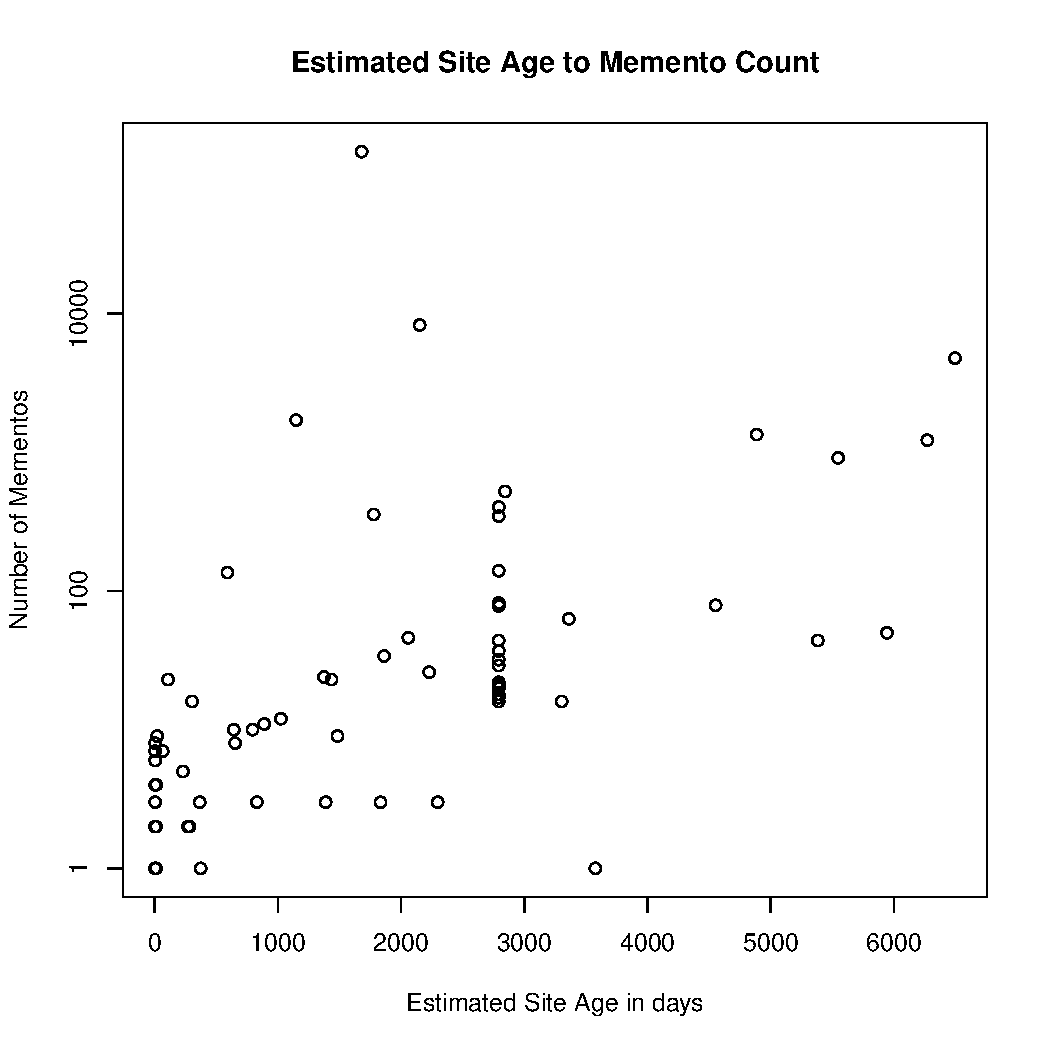
\includegraphics[scale=.85]{q3/ecd_mementos.pdf}}
\caption{Estimated Age to Memento Count}
\label{fig:ecdgraph}
\end{figure}